\documentclass{article}
\usepackage[utf8]{inputenc}
\usepackage{amsmath}
\usepackage{mathtools}
\usepackage{amsthm}
\usepackage{graphicx}
\usepackage{tabularx}
\usepackage{mathtools}
\usepackage{mathrsfs}
\usepackage{enumerate}
\usepackage{amssymb}
\usepackage{accents}
\usepackage{commath}
\usepackage{yfonts}
\usepackage{float}
\usepackage{array}
\usepackage{algorithm}
\usepackage{algpseudocode}
\usepackage{listings}

\title{Stat3001 Assignment 2}
\author{Dominic Scocchera}
\date{April 2023}

\newtheorem{theorem}{Theorem}
\newtheorem{corollary}{Corollary}
\newtheorem{lemma}[theorem]{Lemma}

\begin{document}
\maketitle
\section*{Q1}
\subsection*{a)}
\begin{algorithm}
\caption{Non-Parametric Bootstrap}\label{alg:cap}
\begin{algorithmic}
\Require sample $x_1,x_2,...,x_n$ from a distribution with density $f$ and mean $\mu$
\State Repeat this K times where in the $k_{th}$ iteration:
\State (1) Resample $x_{1k}^{*},x_{2k}^{*},...,x_{nk}^{*}$ from the original data  $x_1,x_2,...,x_n$
\State (2) Compute $\bar{x}_{k}^{*}-\bar{x}$, where $\bar{x}_{k}^{*}=\frac{1}{n}\sum_{i=1}^{n}x_{ik}^{*}$ is the sample mean of the $k_{th}$ bootstrap sample
\State Then $\mathbb{P}(|\bar{X}-\mu|>2)$ can be approximated by $\frac{1}{K}\sum_{i=1}^{K}|\bar{x}^{*}_{k}-\bar{x}|\mathbf{1} _{|\bar{x}^{*}_{k}-\bar{x}|>2}$
\end{algorithmic}
\end{algorithm}
\subsection*{b)}
\begin{algorithm}
\caption{Parametric Bootstrap}\label{alg:cap}
\begin{algorithmic}
\Require sample $x_1,x_2,...,x_n$
\State Estimate $\bar{x}=\frac{1}{n}\sum_{i=1}^{n}x_i$ and $\bar{\sigma^2}=\sqrt{\frac{1}{n}\sum_{i=1}^{n}(x_i-\bar{x})^2}$
\State Repeat this K times where in the $k_{th}$ iteration:
\State (1) Draw a sample $x_{1k}^{*},x_{2k}^{*},...,x_{nk}^{*}$ from the distribution $N(\bar{x},\bar{\sigma^2})$
\State (2) Compute $\bar{x}_{k}^{*}-\bar{x}$, where $\bar{x}_{k}^{*}=\frac{1}{n}\sum_{i=1}^{n}x_{ik}^{*}$ is the sample mean of the $k_{th}$ bootstrap sample
\State Then $\mathbb{P}(|\bar{X}-\mu|>2)$ can be approximated by $\frac{1}{K}\sum_{i=1}^{K}|\bar{x}^{*}_{k}-\bar{x}|\mathbf{1} _{|\bar{x}^{*}_{k}-\bar{x}|>2}$
\end{algorithmic}
\end{algorithm}
\subsection*{c)}
We have the following CDF and ECDF:
\begin{center}
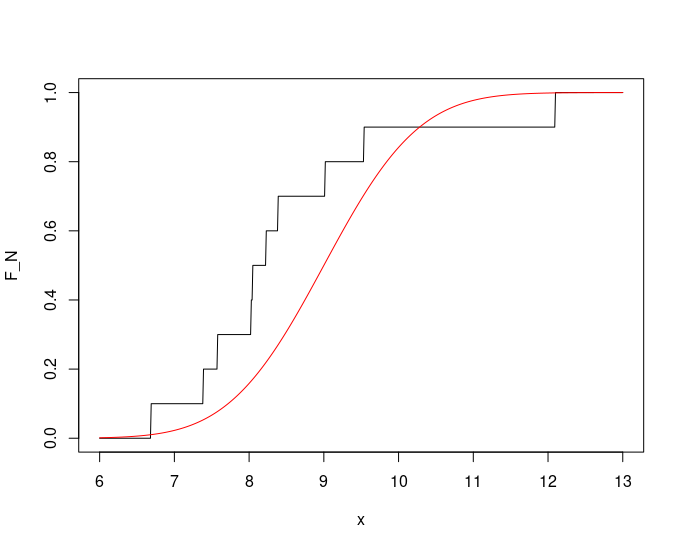
\includegraphics[scale=0.7]{cdf.png}
\end{center}
We perform the Kolmogorov-Smirnov test:
\begin{align*}
\mathbb{H}_0&: \text{The data follows a N(9,1) distribution}\\
\mathbb{H}_1&: \text{The data does not follow a N(9,1) distribution}\\
\end{align*}
The test stastic is:
$$D_n=\max_{1\leq i\leq N}\left[F(x_i)-\frac{i-1}{N},\frac{i}{N}-F(x_i)\right]=0.4290691$$
We let our significance level $\alpha=0.05$. The p-value is 0.03494. This is below the significance level so we reject the null hypothesis. Below is the code used.
\begin{lstlisting}
#data
x = c(8.23, 7.58, 7.39, 9.02, 6.69, 8.05, 8.38, 8.03, 9.54, 12.10)
n = length(x)
#calculate Fn and F
xgrid = seq(floor(min(x)), ceiling(max(x)), by=0.01)
Fn = c()
for(i in 1:length(xgrid)) Fn[i] = mean(x <= xgrid[i]) 
plot(xgrid, Fn, type="n", xlab="x", ylab="F_N")
lines(xgrid, Fn)

#add the true cdf
cdf <- pnorm(sort(xgrid), mean=9, sd=1)
lines(xgrid, cdf, col="red")

#simulate Dn
dn = NULL; K = 100000;
for(k in 1:K) {
  u = runif(n, min=0, max=1);  #random uniform sample
  i = 1:n;                     #index
  u.sorted = sort(u);          #sort u from smallest to largest
  dn[k] = max( max(abs(u.sorted-i/n)), max(abs(u.sorted-(i-1)/n)) ) 
}
#test statistic
dn.max = max(abs(Fn-cdf)); dn.max
#p-value
p.value= mean(dn >= dn.max); p.value
\end{lstlisting}
\section*{Q2}
Recall in Tutorial Sheet 4 Question 4, we implemented a Gibbs sampler to draw samples $\bold{X}=(X,Y)^T$ from the bivariate normal distribution $N(\bold{0},\Sigma)$ where $\bold{0} = (0, 0)^T$ and $\Sigma$ is given below. We describe a random walk Metropolis-Hastings algorithm to draw samples from this bivariate distribution, using the proposal density $N(\bold{0}, \Phi)$, where
$$\Sigma=\begin{pmatrix}
1 & \rho\\
\rho & 1\\
\end{pmatrix}, 
\Phi=\begin{pmatrix}
a^2 & 0\\
0 & b^2\\
\end{pmatrix}$$
Here a and b are constants.
\begin{algorithm}
\caption{Metropolis-Hastings random walk}\label{alg:cap}
\begin{algorithmic}
\Require starting state $\bold{X}_0=\bold{0}$
\State Repeat N times to get N sets of sample from $N(\bold{0}, \Sigma)$ where in the $i_{th}$ iteration:
\State 1) Generate $\bold{Z}$ from $N(\bold{0},\Phi)$, where $\bold{Z}=(z_1,z_2)^T$
\State 2) Calculate the proposal $\bold{Y}=\bold{X}_n+\bold{Z}$, here $\bold{X}_n$ is the current state
\State 3) Evaluate the acceptance probability $\alpha(\bold{X}_n,\bold{Y})=\min\left\{\frac{f(\bold{Y})}{f(\bold{X}_n)},1\right\}$, here $f$ is the joint pdf of the $N(\bold{0},\Sigma)$
\State 4) Generate $U\sim\bold{U}(0,1)$ and calculate $\bold{X}_{n+1}=\begin{cases}
\bold{Y} & \text{if } U\leq\alpha(\bold{X}_n,\bold{Y})\\
\bold{X}_n & \text{else}
\end{cases}$
\newline
\Return $\bold{X}_n$
\end{algorithmic}
\end{algorithm}
\section*{Q3}
We have the density:
$$f(x, y, z)\propto {z\choose y}x^{\alpha+y-1}(1-x)^{\beta+z-y-1}\frac{\gamma^z}{z!}$$
For $0<x<1$, $y=0,1,2,...,z$ , and $z=0,1,2,...$, and where $\alpha>0$, $\beta >0$ and $\gamma>0$ are constants.
\newline\newline
We want to derive a Gibbs sampler.
\newline\newline
The conditional for x is:
\begin{align*}
f_1(x|y,z)&=\frac{f(x,y,z)}{f(y,z)}\\
&\propto f(x,y,z)\\
&\propto x^{\alpha+y-1}(1-x)^{\beta+z-y-1}\\
&\propto \frac{\Gamma(\alpha+\beta+z)}{\Gamma(\alpha+y)\Gamma(\beta+z-y)}x^{\alpha+y-1}(1-x)^{\beta+z-y-1}\\
\end{align*}
The conditional for y is:
\begin{align*}
f_1(y|x,z)&=\frac{f(x,y,z)}{f(x,z)}\\
&\propto f(x,y,z)\\
&\propto {z \choose y}x^y(1-x)^{z-y}
\end{align*}
The conditional for z is:
\begin{align*}
f_1(z|x,y)&=\frac{f(x,y,z)}{f(x,y)}\\
&\propto f(x,y,z)\\
&\propto {z\choose y}(1-x)^z\frac{\gamma^z}{z!}\\
&=\frac{z!}{y!(z-y)!}\frac{((1-x)\gamma)^z}{z!}\\
&\propto \frac{((1-x)\gamma)^ze^{-(1-x)\gamma}}{z!}\\
\end{align*}
So our Gibbs sampler is:
\begin{algorithm}
\caption{Gibbs Sampler}\label{alg:cap}
\begin{algorithmic}
\Require $\alpha,\beta,\gamma > 0$, $0<x_0<1$, $y_0=0,...,z_0$, $z_0=0,1,2,...$
\State $x_{t+1}\sim\text{Beta}(\alpha+y_t,\beta+z_t-y_t)$
\State $y_{t+1}\sim\text{Bin}(z_t,x_{t+1})$
\State $z_{t+1}\sim\text{Poi}((1-x_{t+1})\gamma)$
\end{algorithmic}
\end{algorithm}
\end{document}